\section{Limpando a Poluição na Web: O Navegador Brave \faShield*}

A Web que usamos hoje não é gratuita; nós pagamos por ela com os nossos dados. Navegadores tradicionais (como Chrome ou Edge) foram projetados para rastrear o que você pesquisa, quanto tempo você olha para uma imagem e o que você pretende comprar. 

\vspace{0.3cm}
\noindent
Como vimos em nossa oficina, o problema não são apenas os \enquote{biscoitos} (cookies) que você aceita. Hoje, as empresas usam técnicas avançadas chamadas de \textit{Fingerprinting} (Impressão Digital do Dispositivo). Elas olham o tamanho da sua tela, a marca do seu celular e a sua bateria para saber quem você é, mesmo no \enquote{Modo Anônimo}.

\vspace{0.3cm}
\noindent
A solução para isso não é parar de navegar pela Web, mas sim usar um \textbf{Escudo Ativo}: o navegador \textbf{Brave}.

\vspace{0.3cm} % Respiro
\begin{figure}[h]
	\centering
	
\includegraphics[width=0.6\textwidth]{imagens/brave_color_darkbackground.png}
	\caption*{(\citeauthor{brave_app} \citefield{brave_app}{version} - Versão oficial)}
\end{figure}

\subsection*{Por que usar o Brave no dia a dia?}

\begin{itemize}
	\item \textbf{Bloqueio Nativo de Anúncios:} Ele remove propagandas chatas de sites e vídeos do YouTube automaticamente.
	\item \textbf{Navegação Web mais Rápida:} Como o celular não precisa baixar os \enquote{espiões} e os banners de propaganda, os sites carregam até 3x mais rápido, economizando a sua franquia de dados 4G.
	\item \textbf{Não requer ser um gênio da informática:} Você não precisa instalar extensões difíceis. É só baixar e usar. O Brave bloqueia as invasões \enquote{de fábrica}.
\end{itemize}

\subsection*{Passo a Passo para Limpar sua Navegação:}

\begin{enumerate}
	\item Abra a loja de aplicativos do seu celular (Play Store ou App Store) e pesquise por \textbf{Brave Browser}. Para facilitar, você pode simplesmente \textbf{tocar nas imagens abaixo} (se estiver lendo no celular) ou \textbf{escanear o QR Code} com a câmera para ser levado direto ao aplicativo oficial.
	
	\vspace{0.3cm} % Respiro
	\begin{center}
		\begin{minipage}{\linewidth}
			
			\begin{minipage}{0.3\linewidth}
				\centering
				\textbf{\textcolor{BraveOrange}{\faAndroid \ Android}}\\[0.2cm]
				\href{https://bfaxke.short.gy/brave-browser-android}{
					
\includegraphics[width=0.8\linewidth]{imagens/qr_brave_android.png}
				}\\[0.1cm]
				{\scriptsize (Toque ou escaneie)}
			\end{minipage}
			\hfill
			\begin{minipage}{0.3\linewidth}
				\centering
				\textbf{\textcolor{NordText}{\faApple \ iOS / iPhone}}\\[0.2cm]
				\href{https://bfaxke.short.gy/brave-browser-ios}{
					
\includegraphics[width=0.8\linewidth]{imagens/qr_brave_ios.png}
				}\\[0.1cm]
				{\scriptsize (Toque ou escaneie)}
			\end{minipage}
			\hfill
			\begin{minipage}{0.3\linewidth}
				\centering
				\textbf{\textcolor{BitwardenBlue}{\faDesktop \ Computador}}\\[0.2cm]
				\href{https://bfaxke.short.gy/brave-desktop}{
					
\includegraphics[width=0.8\linewidth]{imagens/qr_brave_desktop.png}
				}\\[0.1cm]
				{\scriptsize (Para Windows/Linux/Mac)}
			\end{minipage}
			
		\end{minipage}
	\end{center}
	\vspace{0.3cm} % Respiro após as imagens
	
	\item Instale o aplicativo \textbf{Brave} (o do Leão Laranja). 
	\item Ao abrir pela primeira vez, ele perguntará se deseja torná-lo seu \enquote{Navegador Padrão}. Escolha \textbf{Sim} (ou \enquote{Definir como padrão}). Isso garante que, ao clicar em um link no WhatsApp, você já abra protegido.
	\item \textbf{Pronto!} Agora, sempre que for pesquisar algo, ler notícias ou abrir o YouTube, use o Brave. 
\end{enumerate}

\subsubsection*{Ocultando Elementos Irritantes da Tela}

Assim como a privacidade do Brave, a função de \enquote{Bloqueio de Elementos} já vem nativamente integrada ao navegador. Você não precisa instalar extensões de terceiros, que frequentemente deixam o celular lento \cite{Brave2026}. Essa ferramenta permite esconder banners, janelas de aviso ou imagens chatas que atrapalham a sua leitura. Vejamos como usá-la no Android.

\vspace{0.3cm}
\noindent
Acesse uma página de sua preferência --- neste exemplo, utilizamos o portal de \textit{Minijogos} \cite{Minijogos2026}. Imediatamente ao abrir um site invasivo como este, o Brave inicia o bloqueio proativo de \textit{scripts}. É crucial entender que a grande maioria desses arquivos invisíveis atua como rastreadores silenciosos (\textit{trackers}), coletando dados sobre o seu hábito de navegação \cite{NIST2017}.

\vspace{0.3cm}
\noindent
Para ocultar algo que o Brave não escondeu sozinho, siga as etapas:
\vspace{0.3cm}

% --- BLOCO DE IMAGENS 1 ---
\noindent
\begin{minipage}{\textwidth}
	\centering
	\begin{minipage}{0.45\textwidth}
		\centering
		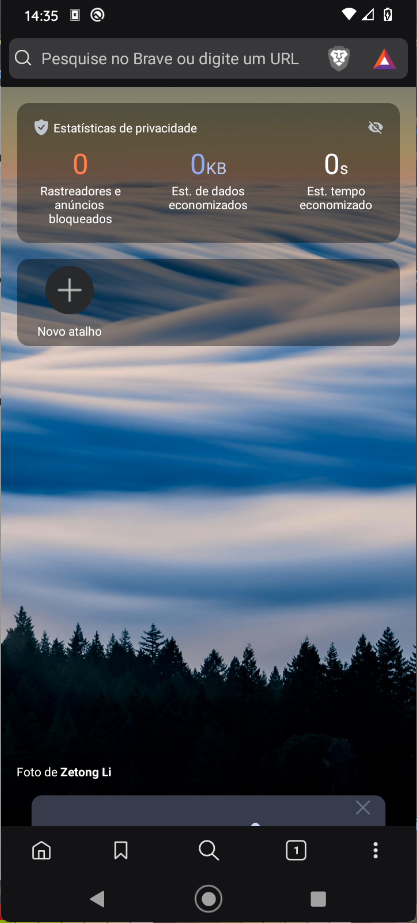
\includegraphics[trim={0cm 15cm 0cm 0cm}, clip, width=\textwidth]{imagens/brave_bloqueio_elementos_01.png}\\[0.2cm]
		\passo{BraveOrange}{1}{Entre em um site}
	\end{minipage}
	\hfill
	\begin{minipage}{0.45\textwidth}
		\centering
		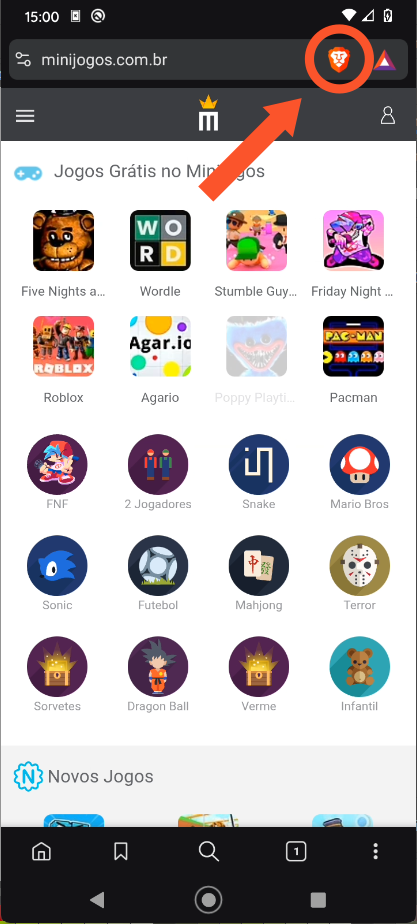
\includegraphics[trim={0cm 15cm 0cm 0cm}, clip, width=\textwidth]{imagens/brave_bloqueio_elementos_02.png}\\[0.2cm]
		\passo{BraveOrange}{2}{Toque no Leãozinho}
	\end{minipage}
\end{minipage}

\vspace{0.3cm}
\noindent
Ao efetuar o Passo 2, o painel de proteção (Escudos) se abrirá.

\vspace{0.3cm}
% --- BLOCO DE IMAGENS 2 ---
\noindent
\begin{minipage}{\textwidth}
	\centering
	\begin{minipage}{0.45\textwidth}
		\centering
		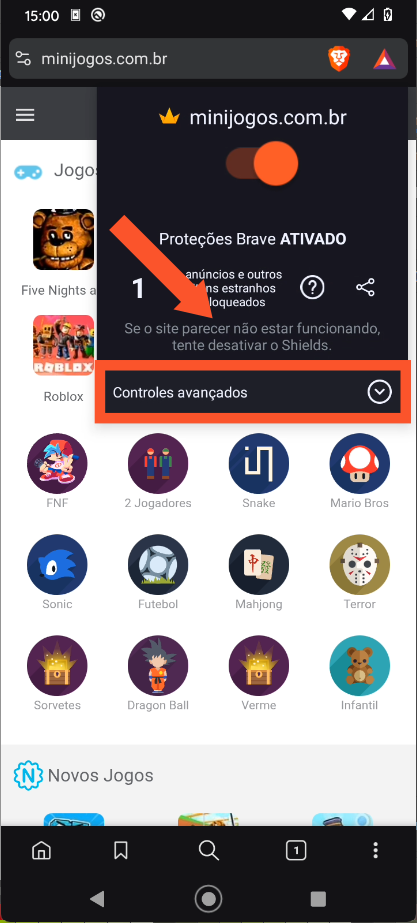
\includegraphics[trim={0cm 0cm 0cm 0cm}, clip, width=\textwidth]{imagens/brave_bloqueio_elementos_03.png}\\[0.2cm]
		\passo{BraveOrange}{3}{Toque em \enquote{Controles Avançados}}
	\end{minipage}
	\hfill
	\begin{minipage}{0.45\textwidth}
		\centering
		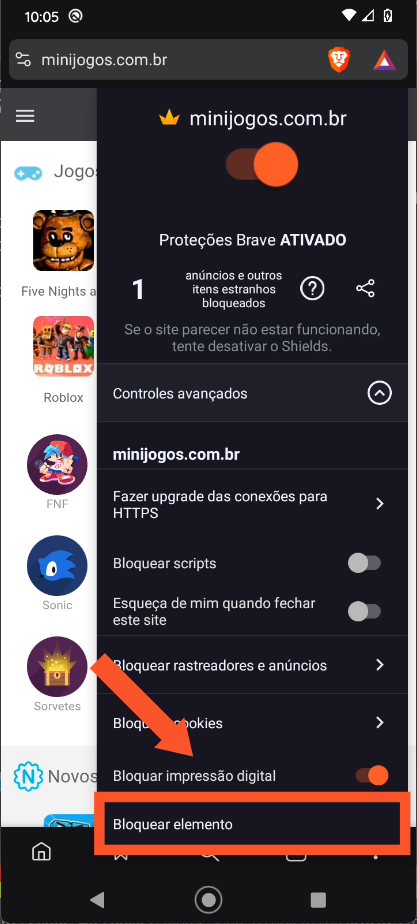
\includegraphics[trim={0cm 0cm 0cm 0cm}, clip, width=\textwidth]{imagens/brave_bloqueio_elementos_04.png}\\[0.2cm]
		\passo{BraveOrange}{4}{Toque em \enquote{Bloquear elemento}}
	\end{minipage}
\end{minipage}

\vspace{0.5cm}

% --- BLOCO DE IMAGENS 3 ---
\noindent
\begin{minipage}{\textwidth}
	\centering
	\begin{minipage}{0.45\textwidth}
		\centering
		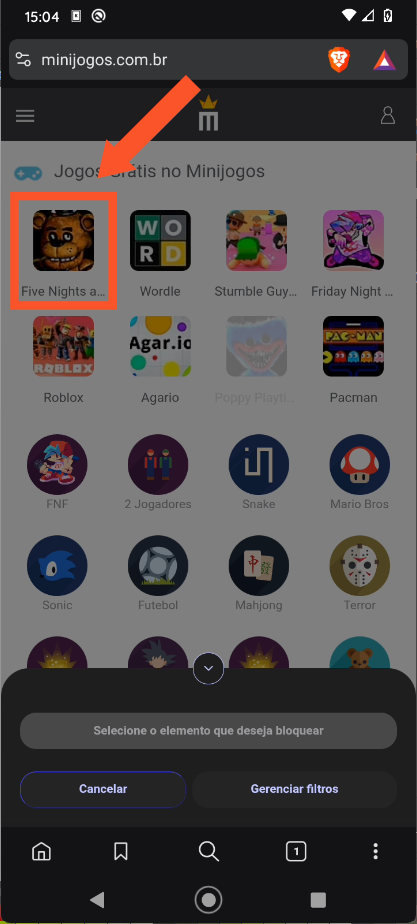
\includegraphics[trim={0cm 0cm 0cm 0cm}, clip, width=\textwidth]{imagens/brave_bloqueio_elementos_05.png}\\[0.2cm]
		\passo{BraveOrange}{5}{Selecione o item \enquote{indesejado}}
	\end{minipage}
	\hfill
	\begin{minipage}{0.45\textwidth}
		\centering
		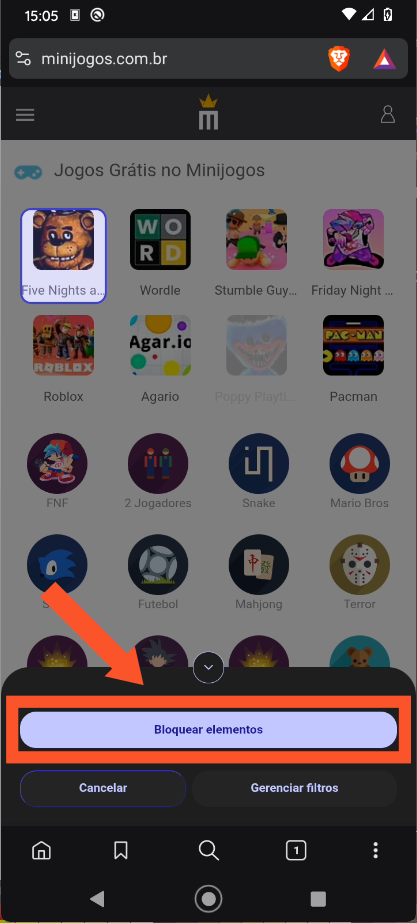
\includegraphics[trim={0cm 0cm 0cm 0cm}, clip, width=\textwidth]{imagens/brave_bloqueio_elementos_06.png}\\[0.2cm]
		\passo{BraveOrange}{6}{Confirme no botão azul}
	\end{minipage}
\end{minipage}

\vspace{0.3cm}
\noindent
Parabéns! O elemento indesejado desapareceu da sua tela. Caso você se arrependa ou esconda o elemento errado sem querer, é muito fácil reverter a ação:

\vspace{0.3cm}
% --- BLOCO DE IMAGENS 4 ---
\noindent
\begin{minipage}{\textwidth}
	\centering
	\begin{minipage}{0.45\textwidth}
		\centering
		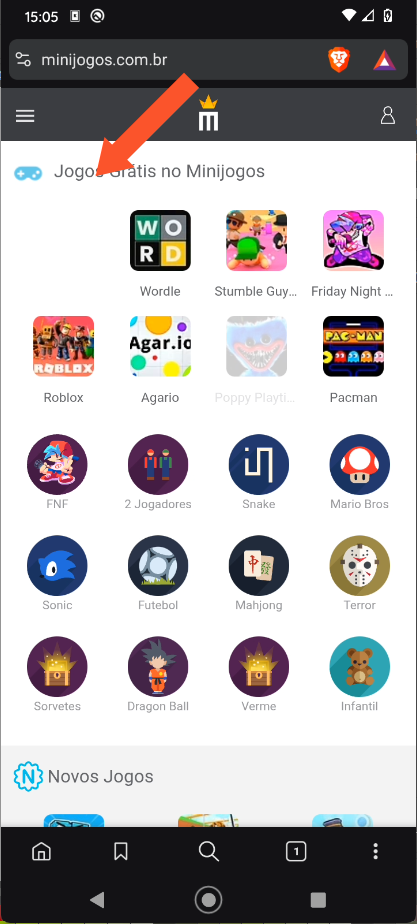
\includegraphics[trim={0cm 15cm 0cm 0cm}, clip, width=\textwidth]{imagens/brave_bloqueio_elementos_07.png}\\[0.2cm]
		\passo{BraveOrange}{7}{O item desapareceu da tela}
	\end{minipage}
	\hfill
	\begin{minipage}{0.45\textwidth}
		\centering
		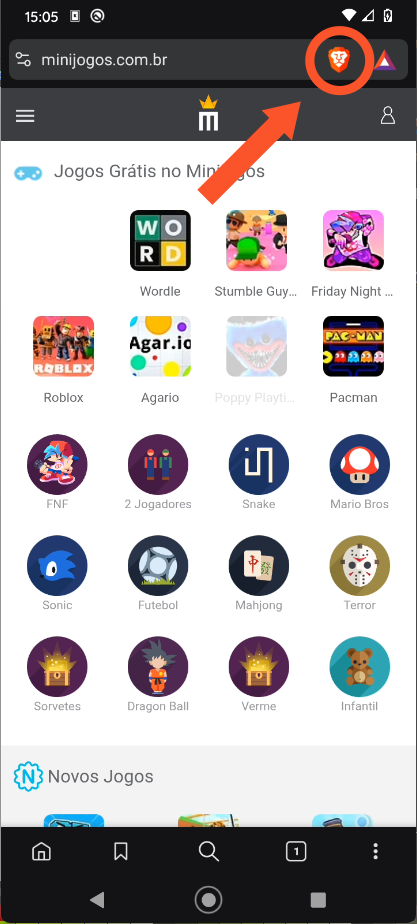
\includegraphics[trim={0cm 15cm 0cm 0cm}, clip, width=\textwidth]{imagens/brave_bloqueio_elementos_08.png}\\[0.2cm]
		\passo{BraveOrange}{8}{Abra o menu do Leãozinho novamente}
	\end{minipage}
\end{minipage}

\vspace{0.5cm}

% --- BLOCO DE IMAGENS 5 ---
\noindent
\begin{minipage}{\textwidth}
	\centering
	\begin{minipage}{0.45\textwidth}
		\centering
		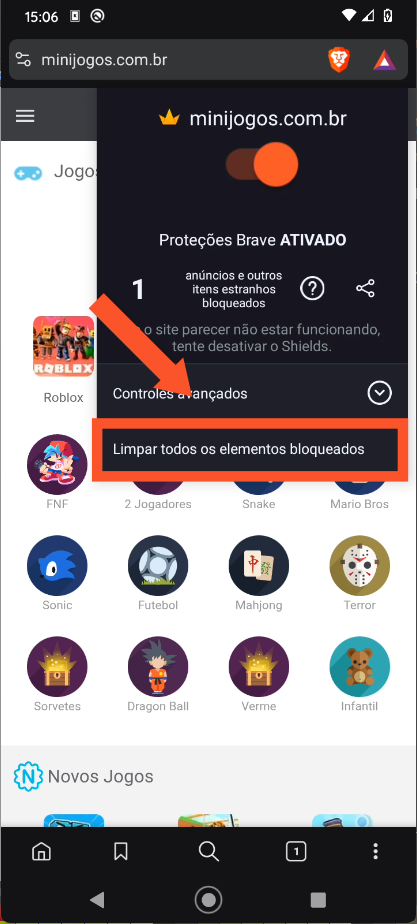
\includegraphics[trim={0cm 10cm 0cm 0cm}, clip, width=\textwidth]{imagens/brave_bloqueio_elementos_09.png}\\[0.2cm]
		\passo{BraveOrange}{9}{Toque em \enquote{Limpar elementos}}
	\end{minipage}
	\hfill
	\begin{minipage}{0.45\textwidth}
		\centering
		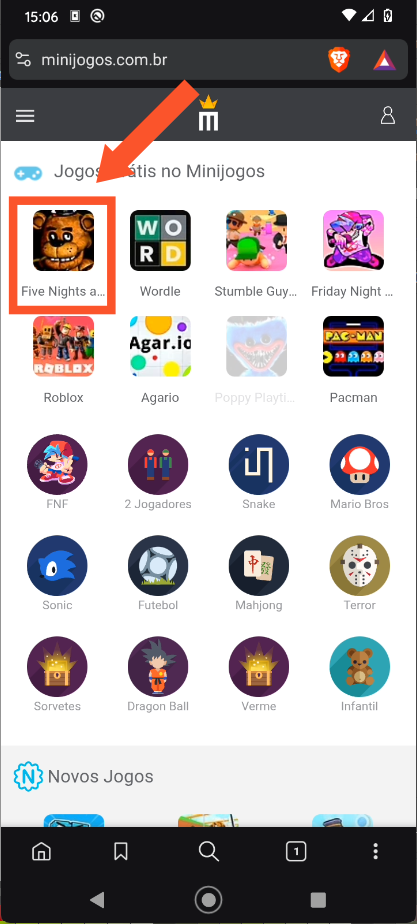
\includegraphics[trim={0cm 10cm 0cm 0cm}, clip, width=\textwidth]{imagens/brave_bloqueio_elementos_10.png}\\[0.2cm]
		\passo{BraveOrange}{10}{O item original retornou à página}
	\end{minipage}
\end{minipage}


\vspace{0.3cm}
\noindent
Explore os \enquote{Controles Avançados} no menu do Leãozinho Corajoso para personalizar ainda mais sua segurança:

\begin{itemize}
	\item \textbf{Fazer upgrade para HTTPS:} Esta opção força a conexão a ser criptografada (o famoso \enquote{Cadeado} na barra de endereço). É uma camada essencial para proteger suas senhas em redes públicas.
	\item \textbf{Bloquear rastreadores e anúncios:} Em sites muito poluídos, mude para \enquote{Agressivo}. O site ficará extremamente limpo e rápido.
	\item \textbf{Bloquear cookies:} Use com cautela. Se ativado para \enquote{Todos}, sites como o Facebook ou o portal da escola vão deslogar a sua conta a cada clique. Deixe na opção padrão de bloqueio de \enquote{Terceiros}.
	\item \textbf{Bloquear impressão digital:} Oculte o modelo do seu celular e a sua placa de vídeo dos sites. É o seu \enquote{Disfarce Digital}.
\end{itemize} 

\begin{tcolorbox}[colback=NordBackground, colframe=BraveOrange, coltext=white, % <--- Isso garante que TODO o texto dentro da caixa seja branco 
	title=\faYoutube \ \textbf{Dica de Ouro para as Mãe}s
	]
	Se você quiser deixar a criança assistindo a desenhos no celular sem o risco de aparecerem propagandas no meio do vídeo, basta abrir o site do YouTube diretamente \textbf{dentro} do navegador Brave. A mágica acontece na hora!
\end{tcolorbox}